\documentclass[sigconf]{acmart}

% Remove/adjust for your submission venue as needed.
% \settopmatter{printacmref=false} % Removes ACM Reference Format
% \renewcommand\footnotetextcopyrightpermission[1]{} % removes copyright text

\usepackage{tikz}
\usetikzlibrary{arrows.meta, positioning}
\usepackage{tabularx}
\usepackage{booktabs}
\usepackage{url}
\usepackage{url}

%\title{Towards Secure, Multitenant, Vendor-Neutral Enterprise RAG on Shared Infrastructure}
\title{Securing the Agent: Vendor-Neutral, Multitenant Enterprise Retrieval and Tool Use}

\author{Varsha Prasad}
\affiliation{%
  \institution{Red Hat AI}
  \city{Boston}
  \country{USA}
}
\email{vnarsing@redhat.com}

\author{Francisco Javier Arceo}
\affiliation{%
  \institution{Red Hat AI}
  \city{Boston}
  \country{USA}
}
\email{farceo@redhat.com}

\begin{abstract}
Retrieval-Augmented Generation (RAG) and agentic AI systems are increasingly prevalent in enterprise AI deployments. However, real enterprise environments introduce challenges largely absent from academic treatments and consumer-facing APIs: multiple tenants with heterogeneous data, strict access-control requirements, regulatory compliance, and cost pressures that demand shared infrastructure.

A fundamental problem underlies existing RAG architectures in these settings: dense retrieval ranks documents by semantic similarity, not by authorization---so a query from one tenant can surface another tenant's confidential data simply because it is the nearest neighbor. We formalize this gap and analyze additional failure modes---including tool-mediated disclosure, context accumulation across turns, and client-side orchestration bypass---that arise when agentic systems conflate relevance with authorization. To address these challenges, we introduce a layered isolation architecture combining policy-aware ingestion, retrieval-time gating, and shared inference, enforced through server-side agentic orchestration. Unlike client-side agent patterns, this approach centralizes tool execution, state management, and policy enforcement on the server, creating natural enforcement points for multitenant isolation and eliminating per-tenant infrastructure duplication.

An open-source, vendor-neutral implementation using Llama Stack---which realizes the Responses API paradigm with server-side multi-turn orchestration---and its Kubernetes Operator demonstrates that secure multitenancy, cost-efficient resource sharing, and the flexibility of modern agentic systems are simultaneously achievable on shared cluster infrastructure.
\end{abstract}

% TODO: update ACM classification.
\begin{CCSXML}
<ccs2012>
 <concept>
  <concept_id>10010147.10010257</concept_id>
  <concept_desc>Computing methodologies~Machine learning</concept_desc>
  <concept_significance>300</concept_significance>
 </concept>
 <concept>
  <concept_id>10002951.10003227.10003351</concept_id>
  <concept_desc>Information systems~Data management systems</concept_desc>
  <concept_significance>100</concept_significance>
 </concept>
</ccs2012>
\end{CCSXML}
\ccsdesc[300]{Computing methodologies~Machine learning}
\ccsdesc[100]{Information systems~Data management systems}

\keywords{Llama Stack, Kubernetes operator, LLM systems, MLOps, LLMOps}

\begin{document}
\maketitle

\section{Introduction}
\subsection{Motivation}
Enterprise adoption of generative AI has evolved beyond simple prompt-response interactions toward agentic systems---AI applications that autonomously reason, use tools, retrieve information, and execute multi-step workflows to accomplish complex tasks~\cite{yao2023react,schick2023toolformer,karpas2022mrkl}.
This evolution reflects a fundamental shift: rather than treating large language models (LLMs) as sophisticated text generators, organizations now deploy them as reasoning engines capable of taking actions in the world.

An API-first paradigm for these systems is to unify multi-turn inference, tool use, and retrieval behind a single endpoint.
OpenAI's Responses API has emerged as a de facto interface pattern for building such systems by providing a unified interface for chat-style inference, tool invocation, retrieval tools, and stateful workflows~\cite{openaiResponsesAPI}.
In parallel, open implementations increasingly expose OpenAI-compatible endpoints to decouple applications from a specific model provider.

However, real-world enterprise deployments differ sharply from the assumptions embedded in consumer-facing APIs and many academic prototypes.
Enterprise environments exhibit characteristics that demand specialized architectural consideration:
\begin{itemize}
  \item \textbf{Multiple tenants:} distinct business units, customers, or partners served from shared infrastructure, with strict isolation requirements.
  \item \textbf{Heterogeneous data:} document collections vary in format, sensitivity classification, and access requirements.
  \item \textbf{Strict access control:} regulatory frameworks require fine-grained governance with auditable access patterns.
  \item \textbf{Operational control:} visibility into agent behavior, tool execution sequences, and data access patterns is required for debugging and compliance, consistent with lessons from production ML engineering~\cite{amershi2019se4ml}.
  \item \textbf{Vendor independence:} lock-in to a single AI provider creates business risk; enterprises require on-prem and hybrid options.
\end{itemize}

Na\"{\i}ve approaches to addressing these requirements replicate the entire agentic stack per tenant: separate vector stores, dedicated inference endpoints, and isolated tool configurations.
This strategy incurs substantial costs --- infrastructure scales linearly with tenants rather than with actual usage --- and creates operational fragmentation that amplifies common ML systems maintenance risks~\cite{sculley2015hiddentechnicaldebt}.

\subsection{Problem statement}
This paper addresses a fundamental tension in enterprise agentic AI deployment:

\begin{quote}
Enterprises require both shared infrastructure for cost efficiency and strict tenant isolation for security and compliance --- while maintaining the flexibility of modern agentic architectures.
\end{quote}

Standard agentic AI deployments exhibit assumptions incompatible with this requirement:
\begin{enumerate}
  \item \textbf{Client-side orchestration:} the application manages the inference--tool--inference loop, distributing security-critical logic to potentially untrusted clients and increasing operational complexity~\cite{amershi2019se4ml}.
  \item \textbf{Homogeneous data access:} retrieval stacks assume uniform access to a corpus; dense retrieval methods (e.g., DPR) optimize similarity ranking rather than authorization~\cite{karpukhin2020dpr}.
  \item \textbf{Implicit trust boundaries:} tool execution is often treated as a capability extension without systematic verification of who may invoke tools or consume tool outputs, despite the centrality of tool use in modern agent designs~\cite{yao2023react,schick2023toolformer,karpas2022mrkl}.
  \item \textbf{Stateless isolation:} requests are treated independently, ignoring how conversation state and cached tool results can leak across boundaries; such hidden couplings are a classic source of ML systems fragility~\cite{sculley2015hiddentechnicaldebt}.
\end{enumerate}

In multitenant settings, these assumptions create serious vulnerabilities.
A document highly similar to a query may belong to a different tenant.
A tool call may access resources outside the user's authorization scope.
Conversation history may accumulate context that crosses security boundaries.

\subsection{Contributions}
This paper makes the following contributions:
\begin{enumerate}
  \item We formalize the problem of \emph{multitenant enterprise RAG} under shared infrastructure, showing why semantic similarity alone (as used by dense retrievers and ANN indexes) is insufficient to enforce isolation and authorization~\cite{karpukhin2020dpr,johnson2017faiss}.

  \item We analyze failure modes of existing RAG and agentic systems in multitenant settings, including cross-tenant retrieval leakage, unauthorized context construction, and policy violations arising from client-side orchestration.

  \item We propose a layered isolation architecture for distributed-scale enterprise RAG that combines policy-aware ingestion, retrieval-time gating, and shared inference to achieve strict tenant isolation without per-tenant duplication of storage or models.

  \item We introduce server-side orchestration as a unifying enforcement layer that centralizes retrieval, tool execution, and state management, reducing the trusted computing base for secure multitenant RAG and aligning with production ML engineering best practices~\cite{sculley2015hiddentechnicaldebt,amershi2019se4ml}.

  \item We present an open-source, vendor-neutral framework based on Llama Stack~\cite{llamastack} and Kubernetes deployment via an operator~\cite{llamastackk8soperator,burns2016borg} that enables pluggable models, vector stores, and tools, demonstrating the feasibility of secure multitenant RAG on shared infrastructure.
\end{enumerate}

\paragraph{Primary sources.}
Llama Stack repository: \url{https://github.com/llamastack/}~\cite{llamastack}.\\
Kubernetes operator repository: \url{https://github.com/llamastack/llama-stack-k8s-operator}~\cite{llamastackk8soperator}.

\section{Background and Related Work}
\subsection{Agentic AI evolution and multitenancy challenges}
LLM application architectures evolved from simple completion APIs to agentic systems that autonomously use tools, retrieve information, and execute multi-step workflows~\cite{yao2023react,schick2023toolformer,karpas2022mrkl}. The Responses API paradigm~\cite{openaiResponsesAPI} unifies chat, retrieval, and tool use but assumes single-tenant deployment.

Multitenancy in agentic AI differs from traditional database or ML serving patterns. Beyond data isolation, agentic systems require policy-aware tool execution, stateful conversation management, and orchestration controls. Production ML systems require systematic lifecycle management~\cite{mlflow} and experience operational fragility when security invariants are distributed across components~\cite{sculley2015hiddentechnicaldebt,amershi2019se4ml}---a problem amplified in agentic deployments where reasoning, retrieval, and tool execution interleave autonomously.

\section{Problem Definition: Multitenant Enterprise Agentic AI}
\subsection{System model and threat analysis}
We formalize the multitenant agentic AI environment: tenants ($T$) share infrastructure, each with associated data, users, tools, and policies. Users possess attributes (roles, clearances, group memberships). Documents live in vector stores with metadata (tenant ownership, classification, access policy). Agent execution follows the tool-using agent pattern~\cite{yao2023react,karpas2022mrkl}: $E = [(i_1, \phi_1, r_1), (i_2, \phi_2, r_2), \dots, (i_n, \emptyset, r_n)]$.

Key threats include: cross-tenant data leakage via retrieval, tool-mediated disclosure, context accumulation attacks, client-side orchestration bypass, and audit failure. Client-side orchestration is fundamentally unsuitable for enterprise multitenancy because it distributes trust to every client, enabling fabricated tool results, unauthorized context injection, and manipulation of conversation state.

\section{Multitenant Agentic AI Challenges and Solutions}
\label{sec:challenges-solutions}

Standard agentic AI deployments exhibit fundamental incompatibilities with enterprise multitenancy. We analyze these failure modes and propose a layered isolation architecture that addresses them.

\subsection{Similarity-authorization gap in retrieval}
Every major RAG framework retrieves documents by semantic similarity using dense retrievers such as DPR~\cite{karpukhin2020dpr} and ANN indexing~\cite{johnson2017faiss}. Similarity is orthogonal to authorization: a document from tenant $B$ may be the most semantically similar result for tenant $A$'s query, yet returning it violates isolation.

Formally, for tenants $T_A$ and $T_B$ sharing corpus $D = D_A \cup D_B$, the isolation invariant requires that only documents with $\mathrm{tenant}(d) = \mathrm{tenant}(u_A)$ be returned. For any similarity threshold $\theta$, there exist queries $q$ such that $\arg\max_{d \in D} \mathrm{sim}(q,d) \in D_B$. Thus similarity-based retrieval cannot enforce tenant isolation without an authorization predicate: $\mathcal{R}(q,u) = \{ d \in D : \mathrm{sim}(q,d) > \theta \wedge P(u,d) = \mathrm{permit} \}$.

\begin{figure}[t]
  \centering
  \resizebox{\columnwidth}{!}{%
  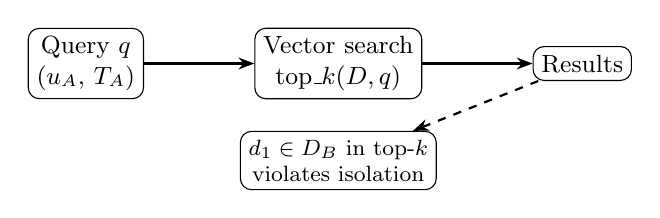
\begin{tikzpicture}[
    box/.style={draw, rounded corners, align=center, inner sep=3pt, font=\small},
    arrow/.style={-{Stealth[length=2.0mm]}, thick}
  ]
    \node[box] (query) {Query $q$\\($u_A$, $T_A$)};
    \node[box, right=14mm of query] (vs) {Vector search\\$\mathrm{top}\_k(D, q)$};
    \node[box, right=14mm of vs] (out) {Results};
    \node[box, below=4mm of vs, font=\footnotesize] (leak) {$d_1 \in D_B$ in top-$k$\\violates isolation};
    \draw[arrow] (query) -- (vs);
    \draw[arrow] (vs) -- (out);
    \draw[arrow, dashed] (out) -- (leak);
  \end{tikzpicture}%
  }
  \caption{Similarity-only retrieval: top-$k$ from shared corpus $D$ can include documents from another tenant ($d_1 \in D_B$), violating isolation.}
  \label{fig:similarity-leak}
\end{figure}

\subsection{Tool-mediated disclosure and client-side orchestration risks}
Agentic systems executing tool sequences~\cite{yao2023react,schick2023toolformer} face unique multitenant threats:
\textbf{Tool-mediated disclosure:} Agents invoke tools with agent credentials rather than end-user authorization, potentially accessing unauthorized data across tenant boundaries.
\textbf{Context accumulation:} Multi-turn conversations persist context without per-turn policy re-validation, enabling cross-tenant data leakage.
\textbf{Client-side bypass:} When orchestration runs client-side, malicious clients can skip authorization checks, manipulate tool invocation, or extract unauthorized data.

These failures stem from distributing security-critical logic outside the trust boundary, consistent with production ML system fragility patterns~\cite{sculley2015hiddentechnicaldebt,amershi2019se4ml}.

\subsection{Layered isolation architecture}
We propose a three-layer solution: policy-aware ingestion, retrieval-time gating, and shared inference.

\textbf{Layer 1: Policy-aware ingestion.} Tenant metadata must be attached at document ingestion time. An ingestion function $\mathcal{I}(d, t) \rightarrow D_t$ tags document $d$ with tenant $t$'s attributes so that every chunk inherits ownership metadata.

\textbf{Layer 2: Retrieval gating.} Two-tier enforcement: (1) resource-level authorization before search, and (2) chunk-level metadata filtering after retrieval. This composes similarity search with mandatory authorization predicates, separating semantic ranking from access control.

\textbf{Layer 3: Shared inference.} The LLM layer is shared across tenants, with isolation enforced at input construction. Since layers 1--2 ensure only authorized content enters prompts, inference can be safely shared, reducing cost from $O(N \cdot M)$ to $O(M)$ for $N$ tenants and $M$ model endpoints.

\subsection{Server-side orchestration as enforcement layer}
Server-side orchestration centralizes retrieval, tool execution, and state management within the trust boundary, eliminating client-side bypass risks. This design aligns with tool-using agent formulations~\cite{yao2023react,karpas2022mrkl} while enabling centralized policy enforcement, audit logging, and state isolation.

Table~\ref{tab:enforcement} maps failure modes to enforcement points.

\begin{table}[t]
  \centering
  \small
  \setlength{\tabcolsep}{3pt}
  \renewcommand{\arraystretch}{1.1}
  \begin{tabularx}{\columnwidth}{@{}l|X@{}}
  \toprule
  Failure mode & Enforcement point \\
  \midrule
  Cross-tenant retrieval leakage & Layer 2 retrieval gating (ABAC + metadata filters) \\
  \midrule
  Context accumulation & Tenant-scoped state storage and per-turn authorization \\
  \midrule
  Tool-mediated disclosure & Server-side tool execution with authorization propagation \\
  \midrule
  Client-side bypass & Server-side orchestration (reduced TCB) \\
  \midrule
  Audit failure & Server-side telemetry and tracing \\
  \bottomrule
  \end{tabularx}
  \caption{Mapping from failure modes to architectural enforcement points.}
  \label{tab:enforcement}
\end{table}

\section{Reference Implementation: Llama Stack}
\label{sec:ref-arch}

Llama Stack~\cite{llamastack} provides an open-source, vendor-neutral implementation of the proposed architecture. Unlike client-side orchestration libraries, Llama Stack executes the complete agentic control loop on the server, creating natural enforcement points for multitenancy and security~\cite{openaiResponsesAPI}.

The framework implements a provider abstraction enabling hybrid deployments: inference providers (vLLM~\cite{kwon2023vllm}, Ollama, OpenAI), vector stores (Chroma, pgvector, Elasticsearch), and tool runtimes (file\_search, web\_search, MCP). Together with open models such as gpt-oss~\cite{openai2025gptoss120bgptoss20bmodel}, this provides a complete open-source alternative to proprietary agentic AI platforms.

\subsection{Multitenant deployment patterns}
The Llama Stack Kubernetes Operator~\cite{llamastackk8soperator} supports multiple deployment topologies:
\textbf{Shared server:} Single instance with logical isolation via ABAC policies and metadata-gated retrieval.
\textbf{Per-tenant instances:} Separate deployments with namespace isolation and shared model backends.
\textbf{Hybrid:} Mixed deployment balancing cost efficiency with stronger isolation for high-security tenants.

Authorization is enforced at API routes, routing resolution, and tool execution, with tenant-scoped state storage and per-turn policy checks preventing cross-tenant leakage.

\section{Kubernetes Deployment}
\label{sec:k8s-operator}

The Llama Stack Kubernetes Operator~\cite{llamastackk8soperator} automates deployment on shared cluster infrastructure~\cite{burns2016borg}. The operator uses a \texttt{LlamaStackDistribution} custom resource to declaratively manage Llama Stack server deployments, supporting multiple topologies: shared instances with logical isolation, per-tenant deployments with namespace isolation, and hybrid approaches balancing cost with security requirements. The operator provides OpenAI-compatible endpoints and optional \texttt{NetworkPolicy} resources for defense-in-depth, layering network-level segmentation on top of application-level ABAC.

\section{Analysis and Discussion}

The layered isolation architecture addresses the failure modes identified above. Cross-tenant retrieval leakage is mitigated by composing similarity retrieval with mandatory policy predicates~\cite{karpukhin2020dpr,johnson2017faiss}. Tool-mediated disclosure is reduced through centralized, policy-gated execution aligned with tool-using agent patterns~\cite{yao2023react,schick2023toolformer}. Context accumulation and state leakage are prevented by tenant-scoped storage and per-turn authorization~\cite{sculley2015hiddentechnicaldebt,amershi2019se4ml}.

Performance depends on the inference backend~\cite{yu2022orca,kwon2023vllm}; predicate pushdown into vector stores is desirable for scale but post-retrieval gating still enforces security invariants.

\textbf{Limitations:} ABAC policies can become complex at scale; metadata filtering timing varies by backend; model prior knowledge is orthogonal to RAG isolation; client-side function tools execute outside the server trust boundary.

\section{Conclusion}
Agentic AI systems introduce multitenancy, access control, and compliance challenges that exceed the assumptions in standard client-orchestrated patterns.
We formalized the insufficiency of similarity-based retrieval for tenant isolation, grounded in dense retrieval and ANN vector search~\cite{karpukhin2020dpr,johnson2017faiss}, and analyzed failure modes of existing RAG and agentic frameworks.
We proposed a layered isolation architecture combining policy-aware ingestion, retrieval-time gating, and shared inference, and argued that server-side orchestration is the unifying enforcement layer that centralizes retrieval, tool execution, and state management and reduces the trusted computing base.
These design choices also reduce operational risk by turning implicit assumptions into enforced invariants, consistent with lessons from production ML systems engineering~\cite{sculley2015hiddentechnicaldebt,amershi2019se4ml}.

Llama Stack~\cite{llamastack} demonstrates that vendor-neutral, open-source tooling can support enterprise-grade multitenancy through provider abstraction, policy enforcement, and a server-side Responses API implementation~\cite{openaiResponsesAPI}. Together with open models such as gpt-oss~\cite{openai2025gptoss120bgptoss20bmodel} and efficient serving via vLLM~\cite{kwon2023vllm}, this provides a complete open-source alternative to proprietary agentic AI platforms.
The Llama Stack Kubernetes Operator~\cite{llamastackk8soperator} enables reproducible deployments on shared cluster infrastructure~\cite{burns2016borg}.
The patterns presented here---server-side orchestration, policy-aware retrieval, defense in depth, and operator-driven infrastructure---provide a foundation for secure, scalable agentic AI deployments that maintain enterprise control over autonomous agent behavior.

\bibliographystyle{ACM-Reference-Format}
\bibliography{references}

\end{document}

